\documentclass{article}
\usepackage{listings}
\usepackage{pdfpages}
\graphicspath{ {.} }

\usepackage{fancyhdr}
\usepackage[pdftex,
	pdfauthor={Aryan Gupta},
	pdftitle={ECGR4181 HW2 Report},
	pdfsubject={Homework Report},
	pdfkeywords={},
	pdfproducer={Latex with hyperref},
pdfcreator={}
]{hyperref}
\usepackage[margin=1in]{geometry}
\hypersetup{colorlinks=true, linkcolor=black,urlcolor=black}
\usepackage[margin=1in]{geometry}
\usepackage{lastpage}
\usepackage[margin=1in]{geometry}
\usepackage{fancyhdr}
\usepackage{amsmath,amsfonts, amsthm}
\usepackage{float}
\usepackage{graphicx}

\lstset{
	basicstyle=\ttfamily,
	columns=fullflexible,
	frame=single,
	breaklines=true,
	postbreak=\mbox{$\hookrightarrow$\space},
}

\begin{document}
	\section{Dinero Prefetcher}
		The Dinero cache simulator also has options to simulate a prefetcher. A prefetcher is an active device that looks for possible data that the program may need in the future and preloads it into the cache or another buffer. This reduces the number of Compulsory misses because the prefetcher attempts to load the data even before the program needs it. The command line switches for the Dinero cache simulator are \verb|-l1-ufetch| which sets the type of prefetcher to use. In our case we used a tagged prefetcher (\verb|-l1-ufetch t|) as stated in the assignment. The next argument is the \verb|-l1-upfdist|, which sets up the prefetcher max stride distance. The last argument used is \verb|-lN-Tpfabort| which sets the abort percentage. 
		
		\begin{table}[H]
			\centering
			\label{din:prefetch_data}
			\begin{tabular}{lll}
			Prefetcher Type & Misses & Total \\
			2 | 50          & 104    & 194   \\
			4 | 50          & 103    & 194   \\
			8 | 50          & 102    & 194   \\
			16 | 50         & 97     & 194   \\
			& & \\
			8 | 10          & 148    & 342   \\
			8 | 20          & 137    & 303   \\
			8 | 25          & 132    & 282   \\
			8 | 75          & 56     & 98   
			\end{tabular}
			\caption{The prefetcher (prefetcher distance | abort percent) and its corresponding misses}		\end{table}
		When the prefetcher distance, the accuracy of the prefetcher did improve, but was not significant to produce any concrete conclusions other than changing the prefetcher distance did not affect this particular trace. Changing the abort percentage gave better results, as the abort rate was decreased the accuracy of the prefetcher increased, possibly because of more space to prefetcher data. This can be seen in Table \ref{din:prefetch_data}
		
	\section{Row/Column Major Test}
		In order to test the Row or Column "major-ness" of my system, a simple test was conducted. 2 2-Dimentional arrays were created and 2 nested loops were used to iterate over the arrays. One loop iterated using row first semantics and the other loop used column first semantics. As seen in Figure \ref{rc:res_graph}, the column major code takes a lot longer than the row major loop when run.
		\begin{figure}[H]
			\label{rc:res_graph}
			\centering
			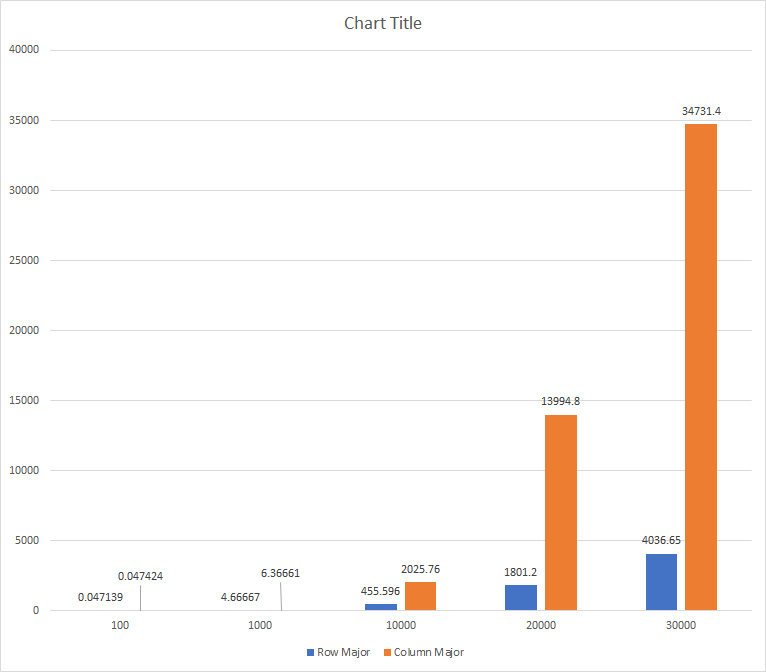
\includegraphics[width=\textwidth]{res_graph.png}
			\caption{The time to iterate over row or column major 2D arrays in milliseconds}
		\end{figure}

\end{document}